% -*-coding: utf-8 -*-
% Держать в начале каждого файла!

\documentclass[a4paper, 12pt]{extarticle}
\usepackage{metod}

\MTDSetPhysSection{Механика}
\MTDSetTitle{Изучениe законов соударения тел}
\MTDDesignator{М--12}
\MTDSetGrade{10}

\MTDSetAuthors{И.~Н.~Грачева, В.~И.~Гребенкин, А.~Е.~Иванов, И.~А.~Коротова,
Е.~И.~Красавина, А.~В.~Кравцов, Н.~С.~Кулеба, Б.~В.~Падалкин,
Г.~Ю.~Шевцова, Т.~С.~Цвецинская}

\MTDSetEditorsGenCase{И.~Н.~Грачевой, А.~Е.~Иванова, А.~В.~Кравцова}

\newcommand{\eps}{\epsilon}
\newcommand{\isum}{\sum\limits_{i=1}^{n}}


\begin{document}

\MTDTitlePage
\MTDInfoPage

\setcounter{section}{12}

\subsection{Цель работы}
Определение коэффициентов восстановления, скорости и энергии при центральном ударе двух шаров, времени и средней силы соударения.\
\subsection{Описание установки}

\begin{figure}[H]
\centering
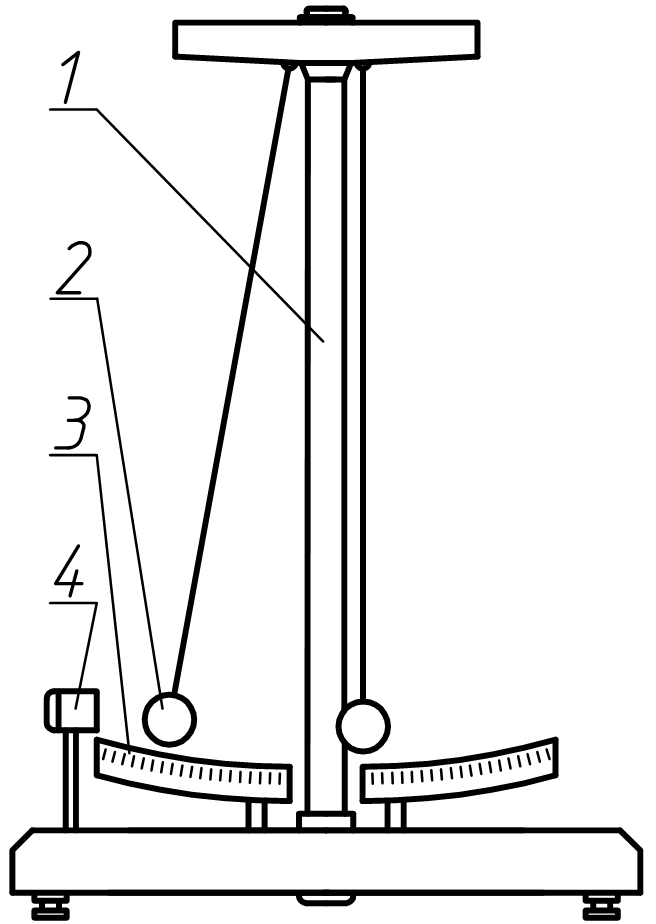
\includegraphics[scale = 0.28, keepaspectratio=true]{M12-CollisionMachine}
\caption{\label{fig:m12-equipment}}
\end{figure}

Схема установки показана на рис.~\ref{fig:m12-equipment}. К штативу~\emph{1} прикреплены два шара~\emph{2}. Углы отклонения подвесов от вертикали определяются по шкалам~\emph{3}. Электромагнит~\emph{4} служит для удержания одного из шаров в отклонённом положении.

\subsection{Основные теоретические сведения}

\begin{figure}[H]
\centering
\begin{minipage}[b]{0.45\linewidth}
\centering
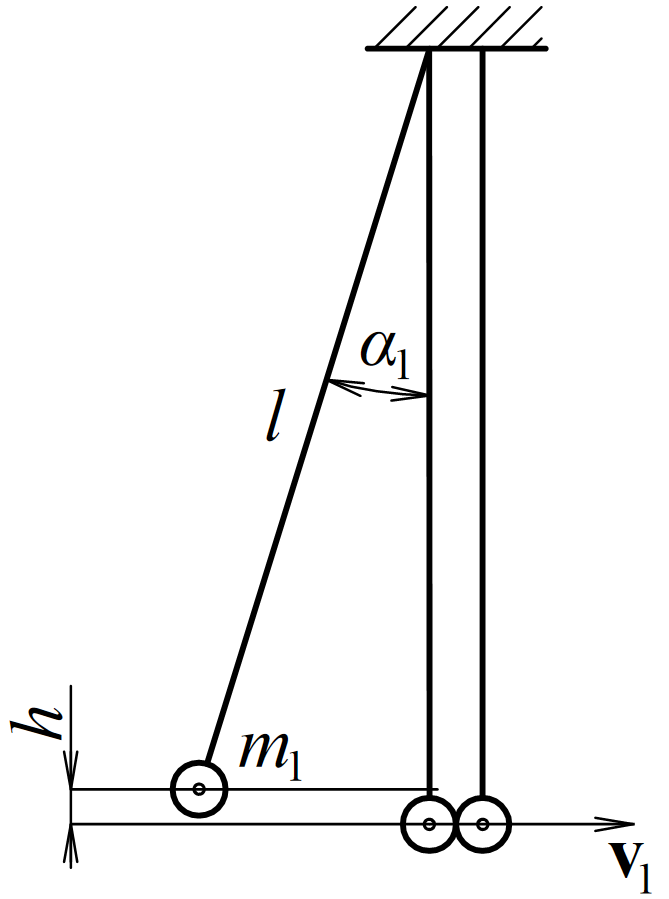
\includegraphics[scale = 0.25, keepaspectratio=true]{M12-PendledumCollision}
\caption{\label{fig:m12-1}} %придумать названия (?)
\end{minipage} \hspace{-1.5cm} % типичный неадекватный способ сдвинуть поближе
\begin{minipage}[b]{0.45\linewidth}
\centering
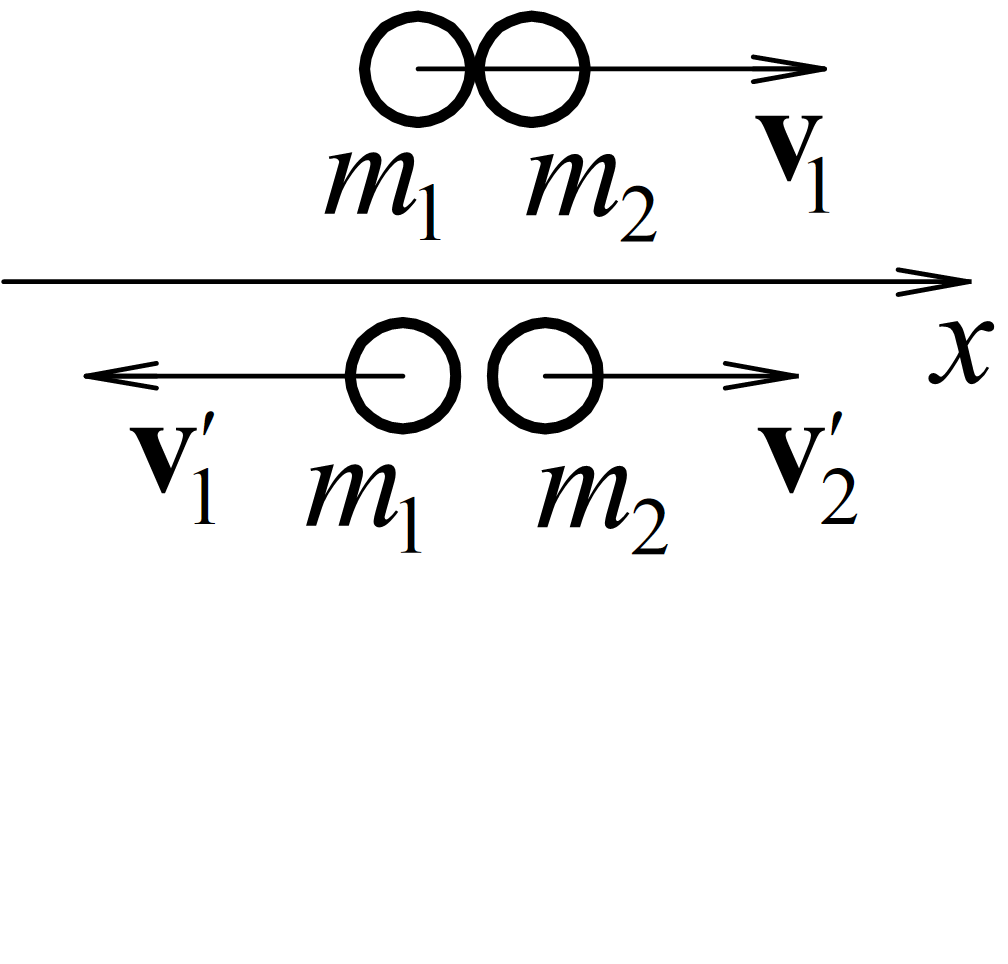
\includegraphics[scale = 0.15, keepaspectratio=true]{M12-BallCollision}
\caption{\label{fig:m12-2}} %придумать названия (?)
\end{minipage}
\end{figure}

Отведём один из шаров (например, левый) на  некоторый угол~$\alpha_1$ и отпустим его без начальной скорости. Отклонённый шар будет двигаться  вниз, при этом его потенциальная энергия будет переходить в кинетическую. Пусть столкновение со вторым шаром происходит в тот момент, когда нить первого шара становится вертикально. По закону сохранения механической энергии (см.~рис.~\ref{fig:m12-1})
\begin{equation}
\label{eq:m12-law-of-conservation}
m_1 g h = \frac{m_1 v_1^2}{2},
\end{equation}
где $m_1$ "--- масса шара, $g$ "--- ускорение свободного падения, $h$ "--- высота шара в отведенном  положении относительно нижней точки траектории, $v_1$ "--- скорость первого шара в нижней точке перед соударением. %убрала \n | "соударением вторым"?! | нужен ли дальше новый абзац? | Имели в виду "перед соударением со вторым", но это вполне очевидно, так что я убрал "вторым". Не нужен.
Из рисунка видно, что
\begin{equation}
\label{eq:m12-alt}
h = l - l \cos \alpha_1,
\end{equation}
где $l$ "--- расстояние от точки подвеса до центра тяжести шара, $\alpha_1$ "--- угол начального отклонения нити. Подставляя~\eqref{eq:m12-law-of-conservation} в~\eqref{eq:m12-alt} и преобразуя уравнение, найдем выражение для скорости через угол начального отклонения: %может наоборот подставляем? | да вроде нормально
\begin{equation}
\label{eq:m12-speed-alt}
\gathered
v_1 = \sqrt{2gh}; \\
h = l (1 - \cos \alpha_1) = 2 \sin^2 \frac{\alpha_1}{2} v_1 = 2 \sqrt{gl} \sin \frac{\alpha_1}{2}.
\endgathered
\end{equation}

Массы шаров подобраны так, чтобы после удара они разлетались в разные стороны. После удара шары получают скорости~$v'_1$  и~$v'_2$  (см.~рис.~\ref{fig:m12-2}), и, разлетаясь, отклоняют нити на максимальные углы~$\alpha'_1$ и~$\alpha'_2$ соответственно. Аналогично соотношению~\eqref{eq:m12-speed-alt} получаем
\begin{equation}
\label{eq:m12-final-speed}
v'_1 = 2 \sqrt{gl} \sin \frac{\alpha'_1}{2}, \ v'_2 = 2 \sqrt{gl} \sin \frac{\alpha'_2}{2}.
\end{equation}

Если удар происходит так быстро, что нити не успевают отклониться на заметный угол, то в направлении горизонтальной оси~$x$ не возникает внешних сил и выполняется закон сохранения импульса в проекции на эту ось: %  ИЗМ: был плохой стиль "Если удар происходит достаточно быстро так, что..." -> "Если удар происходит так быстро, что..." (Вероятно, сначала хотели написать "Достаточно быстро для того, чтобы нити не успели...", но передумали).
\begin{equation}
\label{eq:m12-momentum}
m_1 v_1 = m_2 v'_2 - m_1 v'_1.
\end{equation}

Коэффициент~$\eps_v$ восстановления скорости определяется как отношение относительной скорости шаров после удара к относительной скорости шаров до удара:
\begin{equation}
\label{eq:m12-eps_v-1}
\eps_v = \frac{v'_\text{отн}}{v_\text{отн}}.
\end{equation}

В данном случае формула~\eqref{eq:m12-eps_v-1} с учетом~\eqref{eq:m12-speed-alt} и \eqref{eq:m12-final-speed} преобразуется к виду: % ИЗМ: запятую поменял на "И", никаких причин не использовать там союз нет
\begin{equation}
\label{eq:m12-eps_v-2}
\eps_v = \frac{v'_2 + v'_1}{v_1} = \frac{\sin \dfrac{\alpha'_2}{2} + \sin \dfrac{\alpha'_1}{2}}{\sin \dfrac{\alpha_1}{2}}.
\end{equation}

Для абсолютно упругого удара $\eps_v = 1$. В случае столкновения реальных шаров удар не является абсолютно упругим и $\eps_v < 1$.

Кроме коэффициента восстановления скорости соударение тел характеризуется коэффициентом~$\eps_W$ восстановления энергии, равным отношению кинетической энергии тел после удара к их кинетической энергии до удара:
\begin{equation}
\label{eq:m12-eps_W-1}
\eps_W = \frac{\dfrac{m_1 v'^2_1}{2} + \dfrac{m_2 v'^2_2}{2}}{\dfrac{m_1 v^2_1}{2} + \dfrac{m_2 v^2_2}{2}}.
\end{equation} %пусть она тоже будет пронумерованной | Я не против :)

Учитывая, что скорость второго шара до удара $v_2 = 0$, и подставляя для скоростей выражения~\eqref{eq:m12-speed-alt}, \eqref{eq:m12-final-speed}, находим формулу для коэффициента восстановления энергии: %ИЗМ: пропущенная запятая после $v_2 = 0:  "что скорость второго шара до удара $v_2 = 0$" -- придаточное предложение к "учитывая"
\begin{equation}
\label{eq:m12-eps_W-2}
\eps_W = \frac{m_1 \sin^2 \dfrac{\alpha'_1}{2} + m_2 \sin^2 \dfrac{\alpha'_2}{2}}{m_1 \sin^2 \dfrac{\alpha_1}{2}}.
\end{equation}

Если известна длительность удара $\tau$, то из второго закона Ньютона по изменению импульса левого шара можно определить среднюю силу взаимодействия между шарами:
\begin{equation}
\label{eq:m12-2nd-newton's-law}
F_\text{ср} = \frac{m_2 v_2}{\tau}.
\end{equation}

\subsection{Порядок выполнения работы}
\begin{enumerate}
\item Подключите электромагнит~\emph{4} и клеммы верхнего кронштейна к электронному блоку.
\item Вставьте шары~\emph{2} в скобы подвеса. С помощью регулировочных опор выставьте основание установки таким образом, чтобы нижние визиры скоб подвеса указывали на нули шкал.
\item Отрегулируйте положение шаров в вертикальной и горизонтальной плоскостях до совмещения верхних визиров скоб подвеса. Регулировка производится с помощью изменения длины подвеса шаров, а также изменения положения узлов крепления нитей на верхнем кронштейне.
\item На пульте блока нажмите кнопку <<СБРОС>>. При этом на табло индикации высветятся нули, на электромагнит будет подано напряжение.
\item Отведите левый шар и зафиксируйте его с помощью электромагнита. Определите начальный угол отклонения первого шара~$\alpha_1$.
\item Нажмите кнопку <<ПУСК>>, при этом произойдет удар шаров. По таймеру блока определите время соударения шаров~$\tau$.
\item Определите время соударения для различных пар шаров по методике, описанной в пп.~4--6.
\item В правую скобу подвеса вставьте алюминиевый шар со стальной вставкой, а в левую "--- латунный или стальной шар.
\item Выполните пп.~4--6. При помощи шкал визуально определите углы отскока шаров $\alpha'_1$  и $\alpha'_2$. Повторите измерения углов отскока не менее  трех раз. (Начальные углы отклонения должны быть равны). Найдите среднее значение каждого из углов~$\alpha'_{1\text{ср}}$ и~$\alpha'_{2\text{ср}}$. Все результаты занесите в таблицу~\ref{tab:m12-res-exp-1}.
\item По формуле~\eqref{eq:m12-speed-alt} определите скорость~$v_1$ первого шара перед ударом. Используя среднее значение углов отскока по формулам~\eqref{eq:m12-final-speed} определите скорости обоих шаров сразу после удара~$v'_1$  и~$v'_2$. Результаты занесите в таблицу~\ref{tab:m12-res-exp-2}. Проверьте выполнение закона сохранения импульса.
\item Используя среднее значение углов отскока по формулам~\eqref{eq:m12-eps_v-2}, \eqref{eq:m12-eps_W-2} определите коэффициенты восстановления скорости и энергии.
\item Используя найденное выше значение $v'_2$, по формуле~\eqref{eq:m12-2nd-newton's-law} определите среднюю силу, с которой шары действуют друг на друга во время удара.

\begin{table}[h]
\caption{\label{tab:m12-res-exp-1}}
\begin{center}
      \begin{tabular}{|>{\centering\arraybackslash} m{1.6cm}|>{\centering\arraybackslash} m{1.6cm}|>{\centering\arraybackslash} m{1.6cm}|>{\centering\arraybackslash} m{1.6cm}|>{\centering\arraybackslash} m{1.6cm}|>{\centering\arraybackslash} m{1.6cm}|}
      \hline
      \multirow{2}*{$\alpha_1,~\degree$} & \multirow{2}*{$\tau$,~\Units{с}} & \multirow{2}*{$\alpha'_1,~\degree$} & \multirow{2}*{$\alpha'_{1\text{ср}},~\degree$} &  \multirow{2}*{$\alpha'_{2},~\degree$} & \multirow{2}*{$\alpha'_{2\text{ср}},~\degree$}  \\
      & & & & & \\ \hline
      & & & & & \\ \cline{3-3} \cline{5-5}
      & & & & & \\ \cline{3-3} \cline{5-5}
      & & & & & \\ \hline
\end{tabular}
\end{center}
\end{table}

\begin{table}[h]
\caption{\label{tab:m12-res-exp-2}}
\begin{center}
      \begin{tabular}{|>{\centering\arraybackslash} m{1.6cm}|>{\centering\arraybackslash} m{1.6cm}|>{\centering\arraybackslash} m{1.6cm}|>{\centering\arraybackslash} m{1.6cm}|>{\centering\arraybackslash} m{1.6cm}|}
      \hline
      \multirow{2}*{$v'_1,~\Units{\text{м}/\text{с}}$} & \multirow{2}*{$v'_2,~\Units{\text{м}/\text{с}}$} & \multirow{2}*{$\eps_v$} & \multirow{2}*{$\eps_W$} &  \multirow{2}*{$F_\text{ср}$,~\Units{Н}} \\ %W слишком большая, мб заменить на маленькую | Не стоит морочиться, не так уж оно и ужасно.
      & & & & \\ \hline
	& & & & \\ \hline
\end{tabular}
\end{center}
\end{table}

\end{enumerate}

\subsection{Контрольные вопросы}
\begin{enumerate}
\item Сформулируйте закон сохранения полной механической энергии.
\item Сформулируйте закон сохранения импульса системы материальных точек.
\item Какой удар называется абсолютно упругим?
\item Сформулируйте закон изменения импульса.
\item Выведите формулу~\eqref{eq:m12-speed-alt}.
\end{enumerate}

\end{document}
